% ****** Start of file apssamp.tex ******
%
%   This file is part of the APS files in the REVTeX 4.1 distribution.
%   Version 4.1r of REVTeX, August 2010
%
%   Copyright (c) 2009, 2010 The American Physical Society.
%
%   See the REVTeX 4 README file for restrictions and more information.
%
% TeX'ing this file requires that you have AMS-LaTeX 2.0 installed
% as well as the rest of the prerequisites for REVTeX 4.1
%
% See the REVTeX 4 README file
% It also requires running BibTeX. The commands are as follows:
%
%  1)  latex apssamp.tex
%  2)  bibtex apssamp
%  3)  latex apssamp.tex
%  4)  latex apssamp.tex
%
\documentclass[%
 %reprint,
%superscriptaddress,
%groupedaddress,
%unsortedaddress,
%runinaddress,
%frontmatterverbose, 
preprint,
%showpacs,preprintnumbers,
%nofootinbib,
%nobibnotes,
%bibnotes,
 amsmath,amssymb,
 aps,
 %pra,
prb,
%rmp,
%prstab,
%prstper,
%floatfix,
showkeys,
]{revtex4-1}

\usepackage{graphicx}% Include figure files
\usepackage{dcolumn}% Align table columns on decimal point
\usepackage{bm}% bold math
\usepackage{color}
\usepackage{tabularx}
\usepackage{fullpage,subfigure,float,psfrag,textcomp,gensymb,tikz,siunitx}
\usepackage{booktabs,multirow, dcolumn}% Align table columns on decimal point
\usepackage{xspace}
\usepackage[bookmarks=true,pdftoolbar=true]{hyperref}
\hypersetup{%
  pdftitle = {Co-Ni-Ga:stability of matensitic phase},
  pdfkeywords = {pdf, hyperref, bookmarks},
  pdfauthor = {Anjana Talapatra}}
 \usepackage[all]{hypcap} 



\begin{document}

	\preprint{APS/123-QED}

	\title{Stability analysis of the martensitic phase transformation in \texorpdfstring{$Co_2NiGa$}{Co2NiGa} Heusler alloy}
	\author{Anjana Talapatra$^{1}$}
	\email{anjanatalapatra@tamu.edu}
	\author{Raymundo Arr\'{o}yave$^{1,2}$}
	\author{Peter Entel$^{3}$}
	\author{Valencia-Jaime I. $^{4,5}$}
	\author{Aldo H. Romero $^{5}$}

	\affiliation{ $^{1}$ Department of Mechanical Engineering, TAMU, USA, 77843}
	\affiliation{$^{2}$ Department of  Materials Science \& Engineering, TAMU, USA, 77843}
	\affiliation{$^{3}$Faculty of Physics and CENIDE, University of Duisburg-Essen, 47048 Duisburg, Germany}
	\affiliation{$^{4}$ CINVESTAV-Quer\'etaro, Libramiento Norponiente No 2000, Real de Juriquilla 76230 Quer\'etaro, M\'exico}
	\affiliation{$^{5}$ Department of Physics, West Virginia University, Morgantown WV 26506, U.S.A.}
	\date{\today}

	\begin{abstract}
		Phase competition and the subsequent phase selection are important characteristics of alloy systems exhibiting numerous states of distinct symmetry but comparable energy. The stoichiometric Co$_2$NiGa Heusler alloy exhibits a martensitic transformation with concomitant reduction in symmetry from a austentic $L2_1$ phase (cubic) to a martensitic $L1_0$ phase (tetragonal). A structural search was carried out for this alloy and it showed the existence of a number of structures with monoclinic and orthorhombic symmetry with ground state energies comparable to and even less than that of the $L1_0$ structure, usually reported as the ground state at low temperatures. We describe these structures and focus in particular on the structural transition path from the $L2_1$  to tetragonal and orthorhombic structures for this material. Calculations were carried out to study the Bain ($L2_1 - L1_0$) and Burgers ($L2_1 - hcp$) transformations. The barrierless Burgers path yielded a stable martensitic phase with  orthorhombic symmetry $(O)$ with energy much lower---beyond the expected uncertainty of the calculation methods---than the known tetragonal $L1_0$ martensitic structure. This low energy structure $(O)$ has yet to be observed experimentally and it is thus of scientific interest to discern the cause for the apparent discrepancy between experiments and calculations. It is postulated that the Co$_2$NiGa Heusler system exhibits a classic case of the phase selection problem: although the unexpected $O$ phase may be relatively more stable than the $L1_0$ phase, the energy barrier for the ($L2_1 - O$) transformation may be much higher than the barrier to the ($L2_1 - L1_0$) transformation. To validate this hypothesis, the stability of this structure was investigated by considering the contributions of elastic and vibrational effects, configurational disorder, magnetic disorder and atomic disorder. The calculations simulating the effect of magnetic disorder/ high temperature  as well as the atomic disorder simulations showed that the transformation from $L2_1$ to $L1_0$ is favored over the Burgers path at high temperatures (large magnetic disorder). These conditions are prevalent upon cooling the material from high temperatures (the usual synthesis route), and this provides a plausible explanation of why $L1_0$ and not the $O$ phase is observed. Other ground states (not observed in experiments but predicted through calculations) are ruled out in terms of symmetry relations as well as through considerations of elastic barriers to their nucleation.
	\end{abstract}

	\keywords{DFT, Co-Ni-Ga}
	\maketitle
%%-------------------------------------------------------------------------------------------------------------------------------------------------%%
\section{Introduction}
\label{Sec:intro}

Over the last few decades, experimental and theoretical research into shape memory alloys (SMAs) has gained momentum due to the need for high - temperature multifunctional materials. Current  applications of SMAs are restricted to below 100 $\degree$C for NiTi -based  and Cu-based alloys  which have transformation temperatures in that range.  To be able to realize the advantages offered by these multi-functional materials in the automotive, aerospace and heavy - machinery industries, there is a requirement for  SMAs with much higher transformation temperatures. CoNiGa is one such promising SMA which is the object of much interest due to its potential as a  magnetic SMA with a thermoelastic transition in the ferromagnetic state \cite{siewert2010electronic}. Cobalt has a large magnetic moment which ensures a high Curie temperature. The CoNiGa alloy is sufficiently ductile, exhibits the shape memory effect (SME), and has excellent super - elastic properties \cite{dai2005superelasticity}.  Additionally, it shows martensitic start ($M_s$) temperatures up to 250 $\degree$C \cite{liu2006effect}.
The CoNiGa alloy with a stoichiometric Heusler - type composition (Co$_2$NiGa) is a primary candidate for applications requiring ferromagnetic shape memory alloys\cite{dogan2011microstructure,canadinc2007role,oikawa2001promising,murakami2002magnetic}.

Heusler alloys may be defined as ternary inter-metallic compounds with a stoichiometric composition X$_2$YZ, with the $L2_1$ crystal symmetry. The $L2_1$ unit cell belongs to the space group $Fm\bar{3}m$ and the whole crystal shows only tetrahedral symmetry. X and Y are transition metals while Z is usually a covalently bonding group III-V element. The Heusler structure is bcc-like as it can be formed from the ordered combination of two binary B2
compounds XY and XZ with CsCl structure \cite{dannenberg2011ab}.
Austenitic Co$_2$NiGa exhibits the Heusler $L2_1$ structure (space group $Fm\bar{3}m$) with two inter - penetrating binary B2 compounds CoNi and CoGa with a CsCl structure. The related inverse Heusler structure (CoNi)CoGa can be described as one in which the Co sub - lattice is occupied by the Ni atom, while the displaced Co atoms sit on the Ni sites. DFT calculations have shown that the inverse Heusler structure competes with the conventional Heusler structure in some cases \cite{yamada2014synthesis}. 

In the Co$_2$NiGa system, there is a martensitic transformation from the ordered cubic $L2_1$ to the non - modulated tetragonal $L1_0$ (AuCu, space group $P4/mmm$, 123) phase.  Modulated martensites which are seen in Ni(Mn,Fe)Ga Heusler alloys, have not been observed in the CoNiGa system \cite{Liu2006145, fichtner2015effects}. The $L2_1$ to $L1_0$ transformation can be described as a tetragonal distortion of the cubic austenitic phase. If one assumes that the transformation occurs with minimal volume change, then it can be described through a Bain path, which essentially transforms a bcc structure into a fcc variant as the c/a ratio of the lattice goes from 1 to $\sqrt{2}$. The Bain path shown in Fig. \ref{burger_bain} (red curves) illustrates the transformation. In the figure, $c/a=1$ corresponds to the $L2_1$ phase, while the minimum at $c/a = \sqrt{2}$ corresponds to the low - symmetry, low - energy martensite $L1_0$ with structural symmetry.  

Along with the Bain mechanism, the body centered cubic (bcc) - hexagonal close packed (h.c.p) transformation is the most commonly observed reconstructive phase transformation in simple crystals. It is  found in about 20 elements \cite{toledano1996reconstructive}.  The mechanism used to describe this transformation is the Burgers path \cite{burger1934}, first proposed for the $\beta - \alpha$ transformation in Zr. When applied to the CoNiGa system, surprisingly, the Burgers path is seen to be a barrier - less transformation that reaches a minimum value at distortions resulting from shuffles and shears. This minimum corresponds to a low-energy martensitic structure  with orthorhombic symmetry (space group 59), referred to as the $O$ structure henceforth which is more stable ( has a lower energy ) than the conventional martensitic $L1_0$ structure. The $O$ phase has yet to be reported in the literature and its absence in experiments cannot be merely explained away using kinetic barrier arguments as the 
transformation clearly can go forward  in a monotonic way, at least under ground state---i.e., low - temperature conditions.

In an effort to explain this unprecedented $O$ phase, an extensive investigation was carried out to provide insight into the phenomenon by exploring the energy landscape around the cubic Co$_2$NiGa composition. A structural search by using the minima hopping method\cite{Goedecker2004} was carried out to explore the energy landscape surrounding the conventional martensitic $L1_0$ structure.  These calculations predicted a number of structures with monoclinic, tetragonal, and orthorhombic symmetries with energies much lower than the $L1_0$ structure as well as the $O$ phase, with energy differences much larger than typical computational errors within the chosen approximations. Various high-throughput databases such as the Materials Project \cite{Materialsproject}, the Open Quantum Materials Database (OQMD) \cite{OQMD}, and Automatic Flow for Materials Discovery (AFLOW) \cite{curtarolo2009aflow} did not yield any of the structures predicted by the minima hopping method (MHM) or the Burgers calculations. This may be attributed to the lesser number of known structures for ternary phases, making predictions based on data mining very difficult beyond binary systems or that those methods have been not used in particular for this type of compound.

Even with the extensive energy landscape exploration, the question as to why the Co-Ni-Ga system undergoes a martensitic transformation to the $L1_0$  phase,- while other lower energy structures, specifically the $O$ phase which may be accessed via the Burgers path, exist still remains to be answered. The question may be addressed in either one of three ways: (i) DFT  within a set of given approximations is inadequate to capture the energetics of the transformations in the  Co-Ni-Ga system; (ii) experiments  have so far been unable to isolate the true  martensitic ground state of the system; (iii) the problem may be resolved by invoking phase competition/phase selection at elevated temperatures as the system cools down from a cubic austenitic state.

In addition to the structural search results, we also present total energy calculations for the Burgers transformation and Bain paths in the conventional Heusler and inverse Heusler Co$_2$NiGa  alloys. It is postulated that the isolation of a low-energy martensitic phase which is more stable than the $L1_0$ martensite via \textit{ab-initio} calculations may be attributed to a classic case of the phase selection conundrum, wherein the Co$_2$NiGa $L2_1$ phase preferentially transforms to the $L1_0$ martensitic phase in spite of other possible structures  which are inaccessible even though their energy is lower. Elastic and phonon calculations  were carried out with the intention of isolating any instabilities due to vibrational or elastic effects .  Finally, the Bain and Burgers paths were recalculated taking into consideration the effect of configurational , magnetic, and atomic disorder. This analysis indicates that there is probably a good explanation  of why we do not  observe the other phases  predicted from the structural 
search.

The organization of this paper is as follows: In Sec. \ref{Sec:computational_details}  the computational details and methodology used to perform the calculations is outlined.  In Sec. \ref{Sec:transformations} the Bain and Burgers transformations are applied to austenitic Co$_2$NiGa and the results are presented.  Sec. \ref{Sec:MHM} outlines the minima hopping method as used in this work and the results obtained  therein. The phase selection hypothesis is presented and calculations carried out to validate it are discussed in Sec. \ref{Sec:analysis}. Finally conclusions are drawn in  Sec. \ref{Sec:summary} and the work done is summarized. 
%%----------------------------------------------------------------------------------------------------------------------------------------------------------------------------------------------------------%%
\section{Computational Details and Methodology}
\label{Sec:computational_details}
	The results presented in this work are \textit{ab initio} calculations carried out to determine the electronic, structural, and elastic properties of Co$_2$NiGa stoichiometric Heusler alloys. The calculations were performed within the framework of density functional theory, as implemented in the Vienna ab initio simulation package (VASP)\cite{Kresse1996}, applying the generalized gradient approximation (GGA) using the Perdew-Wang 1991 (PW91) functional \cite{Perdew1992}. Single - parameter Burgers path calculations were also carried out using the local density approximation (LDA) \cite{LDA}. The electronic configurations of the relevant elements were realized using  the projector augmented wave (PAW) pseudo-potentials formalism \cite{blochl1994paw}. Brillouin zone integrations were performed using a Monkhorst-Pack mesh \cite{monkhorst1976} with at least 5000 $k$ points per Brillouin zone or cell. Full relaxations were realized by using the Methfessel-Paxton smearing method of order 1 \cite{methfessel1989}, and self-consistent static calculations were carried out  with the tetrahedron smearing method with Bl\"{o}chl  corrections \cite{blochl1994improved}. A cutoff energy of 350 eV was used for all the  Bain and Burgers path calculations and spin polarizations were accounted for as well. Convergence of the electronic structure was assumed, when changes between two consecutive steps fell below $10^{-7} eV$.

	The elastic constants were calculated by imposing a set of strains $\epsilon=( \epsilon_{1}, \epsilon_{2}, \epsilon_{3}, \epsilon_{4}, \epsilon_{5}, \epsilon_{6})$ 
	on the crystal structure \cite{ganeshan2009effect,ganeshan2009elastic,shang2010first,le2002symmetry,duong2011ab}. The stresses ($\sigma_{i}$) resulting from the change in energy due to the deformation are calculated. By application of  Hooke's law $\sigma_{i}=C_{ij}\epsilon_{j} $, the stiffness tensor $C_{ij}$ may be computed.
	The bulk modulus (B) is calculated by\cite{duong2011ab}:
		\begin{align}
		B = \dfrac{2}{9}\left({C_{11}+C_{12}+ 2C_{13}+ \dfrac{C_{33}}{2}}\right) 
		\end{align}
	The shear modulus is calculated using the Voigt approximation \cite{duong2011ab},
		\begin{align}
		G = \dfrac{1}{15}\left(2C_{11} + C_{33} -C_{12} -2C_{13}+ \right) +
		\dfrac{1}{5} \left( 2C_{44} + \dfrac{1}{2} (C_{11}-C_{12})\right) 
		\end{align}
	while Young's modulus is computed by \cite{duong2011ab}
		\begin{align}
		E = \dfrac{9BG}{3B+G}
		\end{align}
	and Poisson's ratio may be calculated as :
		\begin{align}
		\nu = \dfrac{E}{2G}-1
		\end{align}
%%----------------------------------------------------------------------------------------------------------------------------------------------------------------------------------------------------------%%
\section{Transformation paths in \texorpdfstring{$Co_2NiGa$}{CO2NiGa} }
\label{Sec:transformations}

The crystallographic relations for the b.c.c-h.c.p transformation were established  by Burgers \cite{burger1934} and can be described as:
\begin{equation}
(110)_{b.c.c} \parallel (0 0 0 1)_{(h.c.p)} \ , \ \ \ \ \;[\bar{1}  1  1]_{b.c.c} \parallel [\bar{2}  1  1  0]_{h.c.p}
\end{equation}
The transformation manifests in the form of two collective movements of atomic planes:
 (i) shearing towards the $[\bar{1} 1 1]$ direction along the $(1\bar{1}2)$  plane transforming the $(110)$ b.c.c plane into the (0001) h.c.p plane, and (ii) shuffling of alternate (110) planes
in the $[0\bar{1} 1 0]$ direction ,with a  constant $(110)$ interplanar distance.
The Burgers mechanism thus involves two distinct and simultaneous structural changes characterized by primary order parameters.

\subsection{1-parameter Burgers path}
\label{Sec:1D_formalism} 

\begin{figure}[htp!]
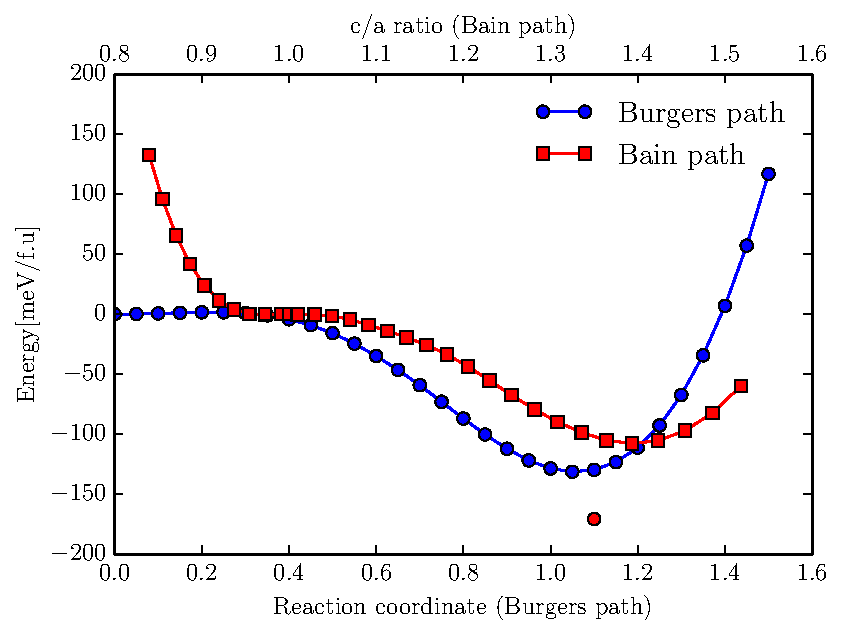
\includegraphics[scale=1.0]{figure_1}
\caption{ Energy profile comparison for Bain and single-parameter Burger  paths in  $Co_2NiGa$ . The minimum along the Burgers path occurs at approximately $\delta =1.1$ ($O$ structure). The single data point in the figure corresponds to the completely relaxed minimum energy structure.}  
\label{burger_bain}
\end{figure}

Friak et al. \cite{friak2008ab} coupled the two degrees of freedom to obtain a single-parameter Burgers path to study the b.c.c-h.c.p transformation in iron \cite{vsob1998ab,vsob1999proceedings,friak2008ab}. This model is modified and applied to the $L2_1 \rightarrow hcp$ transformation in this work.
Proceeding in a manner similar to \cite{friak2008ab},the simplest transformation is accomplished using  an orthorhombic basis applied to a 1x2x1 supercell of a 4-atom unit cell. For a $L2_{1}$ lattice constant \textit{a} , the orthorhombic lattice parameters will be
\begin{align}
 a_0 = \dfrac{\sqrt{2}a}{{s(\delta)}^{1/3}}; \ \ \ \ \ \ \;
 b_0 = a\left(\dfrac{\delta(2\sqrt{3} - 3\sqrt{2})}{6} +\dfrac{ \sqrt{2}} {2} \right); \ \ \ \ \ \ \;
 c_0 = a\left( \dfrac{\delta (2\sqrt{2} - 3)}{3} + 1\right)
\end{align}
where:
\begin{align}
s(\delta) = \sqrt{2} \;\left( \dfrac{\delta(2\sqrt{3} - 3\sqrt{2})}{6}  + \dfrac{\sqrt{2}}{2}\right)\cdot \left( \dfrac{\delta(2\sqrt{2} - 3)} {3} + 1\right)
\end{align}
Here, $\delta =0 $ corresponds to the $L2_1$ phase and $\delta =1$represents the $hcp$ phase. 
Correspondingly, the angle in the (110) $L2_1$ planes evolves from $\theta=109.47 ^\circ $ to $\theta=120 ^\circ $. The $(110) \ L2_1$ planes are transformed to the $(0001) \ hcp $ stacking  planes. 

In Fig.\ref{burger_bain}, we present the profile of the differential energy ($\delta E$) along the Bain path and single-parameter Burgers paths for $CoNiGa$ . For the Burgers path, $\delta =1$ corresponds to the perfect $hcp$ lattice type. It is seen that the minimum along the Burgers path occurs at approximately $\delta =1.1$. The single data point in the figure corresponds to the completely relaxed minimum energy structure. The energy of this structure is noted to be further lowered by about $50 \ meV $ upon complete relaxation. 

\subsection{2-parameter Burgers path}
\label{Sec:2D_formalism}
 When both degrees of freedom are considered, this gives rise to the Burgers surface which determines the energy field for the transformation. Nishitani et al \cite{nishitani2001first} described the b.c.c-h.c.p transformation in Ti using the Burgers surface by performing first-principle calculations using a two-parameter model corresponding to the above mentioned two degrees of freedom. 

 In order to model the Burgers surface of the Co$_2$NiGa and Co$_2$NiAl Heusler alloys, keeping the atomic volume constant, the most rigorous transformation path is achieved by using an orthorhombic basis (space group :CmCm, \#59, Pearson symbol:$oS4$) in conjunction with an 8-atom unit cell. The evolution of the basis vectors and atom positions gives rise to a two-dimensional parameter space ( $\delta, \eta$), where $\delta_1$ accounts for the basal shear and $\eta$ for the shuffle. For a $L2_{1}$ lattice constant \textit{a} , the orthorhombic lattice parameters will be
\begin{align}
  a_0 =a\sqrt{2}\ ; \ \ \ \ \; b_0 =2a/s(\delta)\ ; \ \ \ \ \; c_0 = a\sqrt{2}s(\delta)
  \end{align}
where:  
\begin{align}
s(\delta) = 1 + \left[\left( \dfrac{3}{2}\right)^{0.25} - 1\right]\delta
\end{align}
The basis vectors are given by $[a_0,0,0],[0,b_0,0],[0,0,c_0]$, with atom positions $(0, 0.25, 0.5)$, $(0, 0.75, 0)$, $(0.5, 0.25, \eta/6)$, $(0.5, 0.75, \eta/6)$, $(0, 0, 0)$, $(0.5, 0.5, 0.5 + \eta/6)$, $(0, 0.5, 0)$ and  $(0.5, 0, 0.5 + \eta/6)$.
The $L_21$ and $hcp$ phases then correspond to (0,0) and (1,1) respectively.

Fig.\ref{Burgers}, shows the Burgers energy surface for the $Co_2NiGa$  Heusler alloy considering a two-parameter Burgers path that takes explicit account for shuffles and shears necessary to transform a bcc lattice into an hcp variant. In the figure, $(0,0)$ corresponds to the $L2_1$ structure and (1,1) corresponds to an hcp-like structure. 


\begin{figure}[htp!]
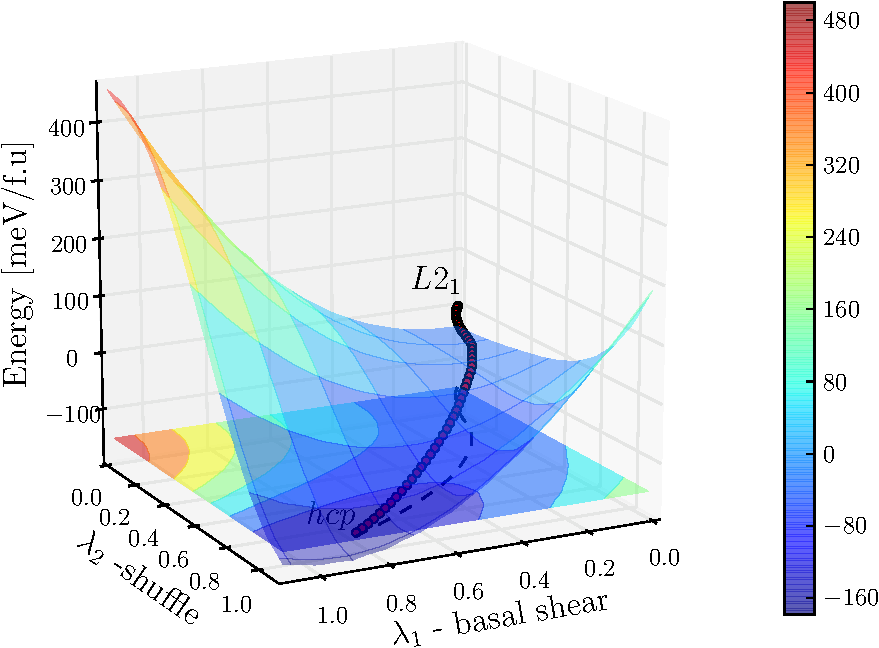
\includegraphics[scale= 1.0]{figure_2}
\begin{picture}(0,0)
\put(-200,200){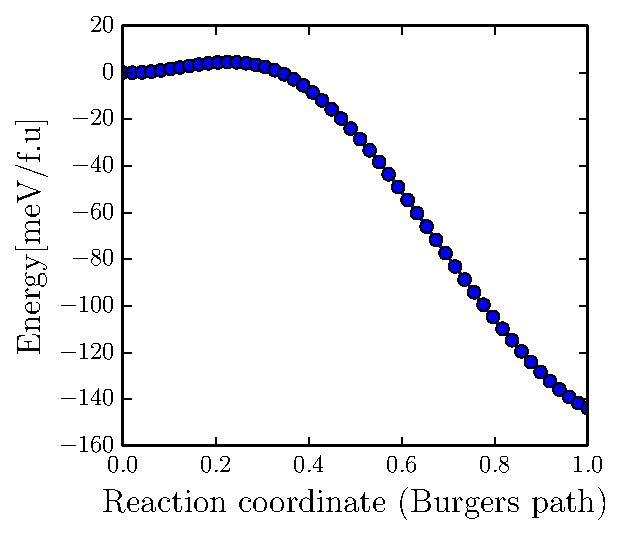
\includegraphics[height = 4cm]{figure_2a}}
\end{picture}
  \caption{Burgers energy surface for $Co_2NiGa$ Heusler alloys. $(0,0)$ corresponds to the $L2_1$ structure and (1,1) corresponds to the hcp structure.Inset: Energy profile for the transformation.} 
  \label{Burgers}
\end{figure}
For these calculations, a 17x17 grid was used and the energy of the intermediate structures at each grid point was calculated using methods detailed in Sec. \ref{Sec:computational_details}. A second-order accurate finite difference scheme was then used to compute the total energy surface. The minimum energy path (MEP) for the Burgers transformation through this energy surface was constructed by using the modified string method \cite{samanta2010modified}. This method allows determination of  the MEP by finding the minimum energy configuration along the hyperplanes normal to the path. The MEP for the Burgers transformation is also indicated along the surface. The inset shows the energy profile of the transformation, which is again barrierless. The energy values for all the different fully relaxed structures along with their lattice parameters  are summarized in Table \ref{tab:CoNiGa_energy}.


\begin{table}[ht]
\caption{Lattice parameters and energy values for  $Co_2NiGa$ and $Co_2NiAl$. Calculations were performed using the  GGA \cite{Perdew1992} approximation. Energy difference is computed relative to the  $L1_0$ structure in $meV/f.u$}
\setlength{\tabcolsep}{0.56cm}
\begin{tabular}{lcccccc}
\hline \hline
Model  & Structure          & Space               & a                         & b                         & c                         & $\delta E$ \\
        &                    & Group               & (\AA)                       & (\AA)                       & (\AA)                       & (meV/f.u)  \\ \hline 
        & $L2_1$             & 225                 & 4.015                     & 4.015                     & 4.015                     & 108.402    \\
        & $L1_0$             & 123                 & 4.364                     & 4.364                     & 3.598                     & 0.000      \\
1-param & \multirow{2}{*}{O} & \multirow{2}{*}{59} & 4.113                     & 5.094                     & 4.397                     & -68.747    \\
2-param &                    &                     & \multicolumn{1}{l}{4.484} & \multicolumn{1}{l}{5.084} & \multicolumn{1}{l}{4.073} &  -118.436  \\
\hline
\end{tabular}
\label{tab:CoNiGa_energy}
\end{table}


From Table \ref{tab:CoNiGa_energy}, it is seen that both the 1-parameter and 2-parameter Burgers paths yield a stable orthorhombic phase appreciably lower in energy than $L1_0$ via barrier-less transformations. 
Subsequently, it was deemed necessary to explore the energy landscape surrounding the $L1_0$ structure by applying the minima hopping methods, results of which are detailed in the following section.
%%----------------------------------------------------------------------------------------------------------------------------------------------------------------------------------------------------------%%
\section{Minima Hopping Method}
\label{Sec:MHM}
Minima hopping calculations were carried out for the Co$_2$-Ni-Ga chemical composition. The basics of the method are described in detail in the original references \cite{Goedecker2004,Amsler2010}. In summary, this method
performs a systematic \textit{ab initio} search for low-enthalpy phases of a given compound, where the only input is the chemical composition and the number of atoms in the simulated cell.
Short Rahman-Parrinello molecular dynamics simulations \cite{parrinello1981polymorphic}, are used to escape from local minima and 
efficient local geometry relaxations were performed to identify stable configurations. The efficiency of the escape step was ensured by aligning the initial atomic velocities within the molecular dynamics along a soft mode direction.
The energy and stresses are obtained by interfacing the method with VASP \cite{Kresse1996}. As in the total energy calculations, the projector augmented wave (PAW) method was used to describe valence and core electrons \cite{blochl1994}. To approximate the exchange-correlation functional we used the
Perdew-Burke-Ernzerhof (PBE) \cite{Perdew1996} generalized gradient
approximation. After the potential structures are found by the minima hopping method, the structure is tightly minimized by using a plane wave cutoff of 550 eV, and the $k$ mesh used to calculate the observables in the Brillouin zone is adapted such that the calculation guaranteed a numerical convergence of the total energy to less than 2 meV/atom. The structures were also re-optimized by using other functionals in accordance with the total energy calculations.

A summary of the results is shown in Table \ref{tab:minima_hopping}. This table shows the energy of all structures using GGA \cite{Perdew1992}, PBE \cite{Perdew1996}, and LDA \cite{LDA} approximations relative to the relaxed  $L1_0$ structure.
It is seen that a number of structures with monoclinic, tetragonal and orthorhombic symmetries are predicted with energies much lower than the $L1_0$ structure. The list also includes the $O$ phase, which was observed in section \ref{Sec:transformations} to result from a Burgers transformation of the original $L2_1$ structure. This shows that a number of low-energy structures theoretically exist in the thermodynamic vicinity of $L1_0$ but have been inaccessible experimentally. Fig. \ref{fig:xrd} shows the simulated x-ray diffraction  spectra for some of the lowest-energy structures, that can be used by the experimentalist to compare with some of our-low energy structures. The transformation mechanisms for all these structures, except the $O$ structure, are unknown. The possibility of considering all possible structural transitions from the $L1_0$ phase to the predicted ones is not the focus of this paper. Instead, we  focus only on the  $O$  structure and conduct a thorough analysis to investigate (i) the 
stability of the structure and (ii) the possible energy barriers which may render these low-energy structures inaccessible.

  \begin{table}
    \caption{Energy difference of the predicted crystal structures in $meV/f.u$ for $Co_2NiGa$ }
    \centering
    \setlength{\tabcolsep}{0.8cm}
    \begin{tabular}{c c c c c} 
        \hline \hline
        \multicolumn{1}{c}{Space} & \multicolumn{ 3}{c}{$\delta E$} & \multicolumn{1}{c}{Structure} \\ 
        \multicolumn{1}{c}{Group} & \multicolumn{1}{c}{GGA} & \multicolumn{1}{c}{PBE} & \multicolumn{1}{c}{LDA} &\multicolumn{1}{c}{}\\ 
        \hline
       123 & 0 & 0 & 0 & $ {L1_0}$ \\ 
       3 & -58.0920 & -21.2160& -67.1520 & monoclinic \\ 
       5 & -55.5360 & -51.1120 & -82.5480 & monoclinic \\ 
       8 & -109.976 & -100.936 & -150.396 &  monoclinic \\ 
       11 & -139.124 & -136.228 & -167.192 & monoclinic\\ 
       12 & -122.636 & -115.444 & -159.772  & monoclinic \\ 
       31 & -104.456 & -99.6720  & -136.620 & orthorhombic \\ 
       40 & -66.2120 & -61.1280 & -91.3280 & orthorhombic \\ 
       44 & -78.9040 & -71.2440    & -117.124 & orthorhombic \\ 
       51 & -68.9520 & -75.6160 & -61.2120 & orthorhombic \\ 
       59 &  -132.536 & -144.816 & -151.376 & ${O}$ \\ 
       63 & -125.012 & -126.512 & -152.972 & orthorhombic \\  
       119 &  -137.296 & -131.360  &  -183.000  & tetragonal \\ 
       139 & -27.9680 & -20.7720 & -67.9200  & tetragonal \\ 
       216 & 83.3960 & 89.4600 & 94.6720 & Inv. Heusler\\ 
       225 & 108.402 & 109.232 & 78.2080 & $L2_1$ \\ 
        \hline
      \end{tabular}
    \label{tab:minima_hopping}
    \end{table}

\begin{figure}[htp!]
  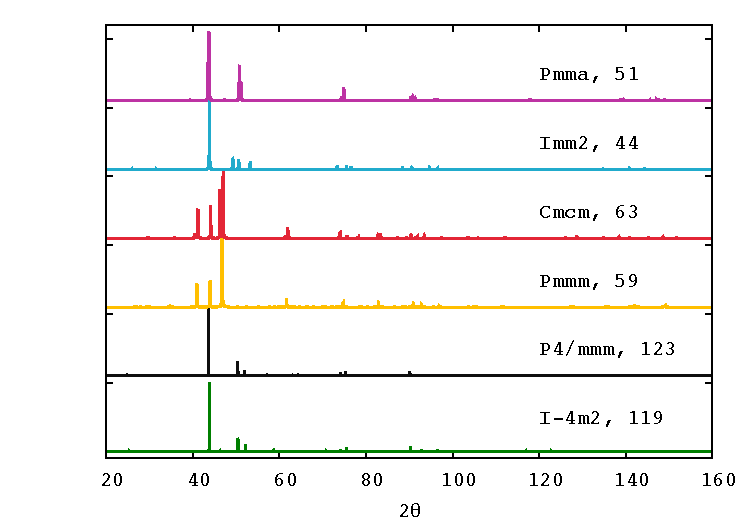
\includegraphics[scale=0.9]{figure_3}
  \caption{Simulated x-ray diffraction spectrum with Cu K$\alpha$ radiation, $\lambda$=1.54178 \AA \  for some of the low-energy structures reported in Table~ \ref{tab:minima_hopping}} 
  \label{fig:xrd}
\end{figure}
%%----------------------------------------------------------------------------------------------------------------------------------------------------------------------------------------------------------%%
\section{Analysis and Discussion}
\label{Sec:analysis}

 \begin{figure}[htp!]
\centering
\subfigure[ $ L2_1 $ - $ O $ ]{
  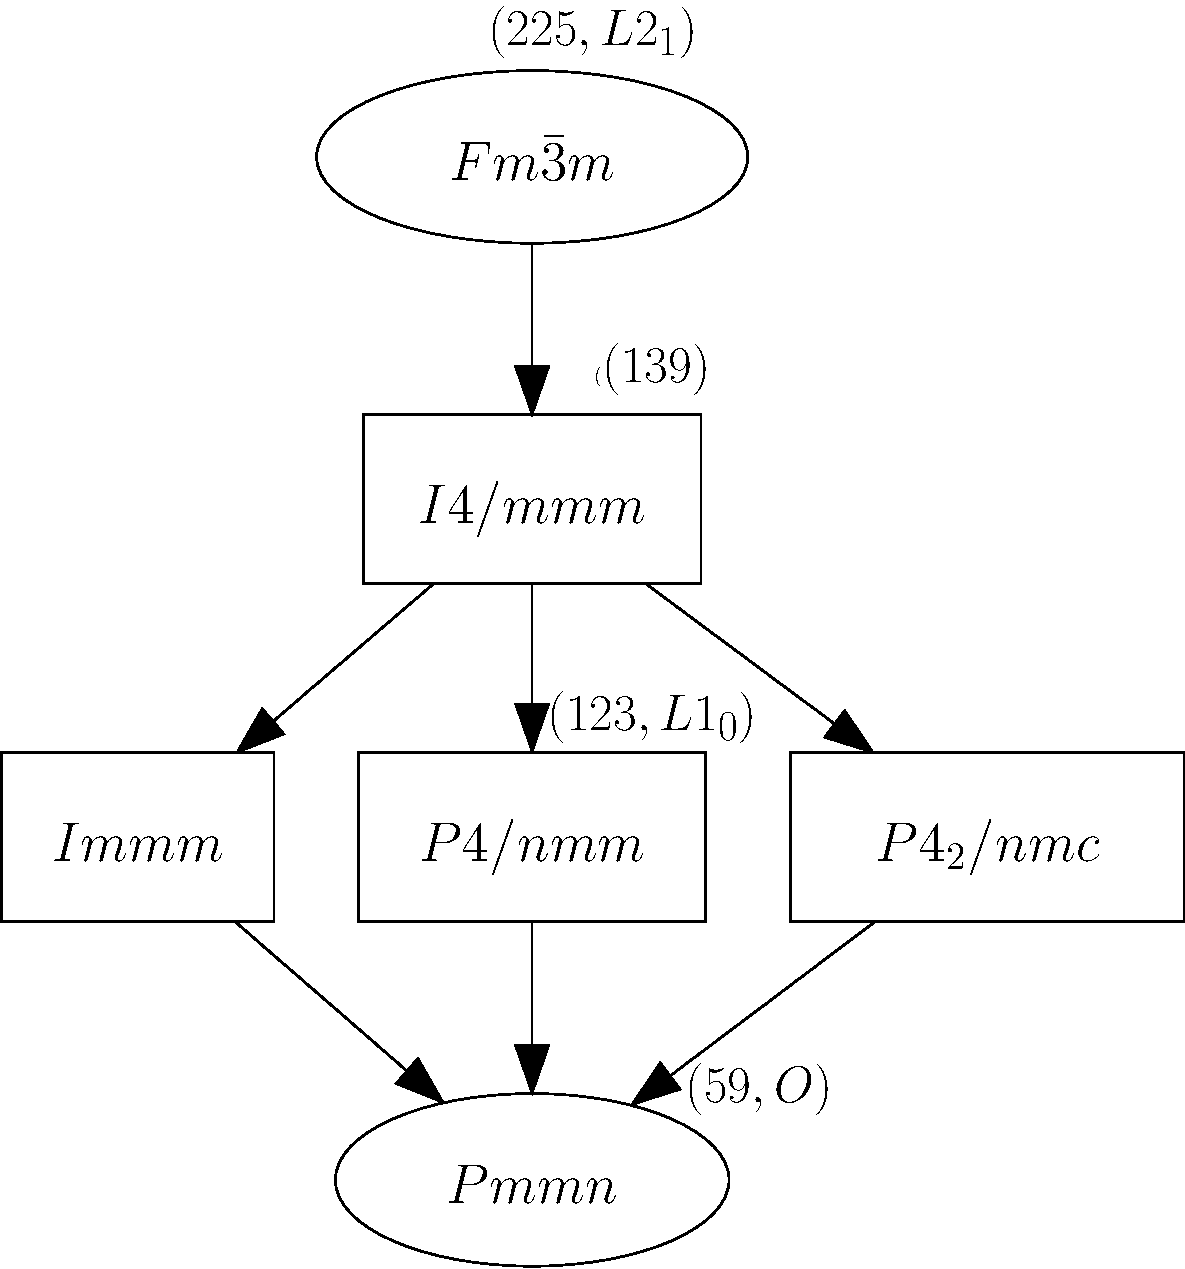
\includegraphics[scale=0.36]{figure_4a}}
  \hspace{1em}
\subfigure[ $ L2_1 $ - $ L1_0 $ ]{
  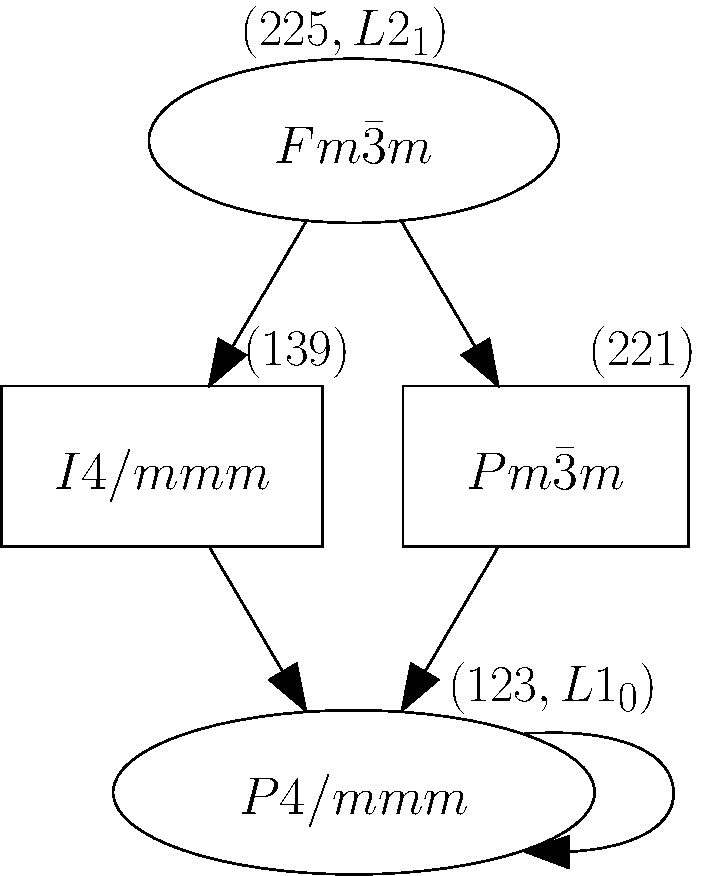
\includegraphics[scale=0.36]{figure_4b}}
  \subfigure[ $ L2_1 $ - $ Cmcm, 63 $ ]{
  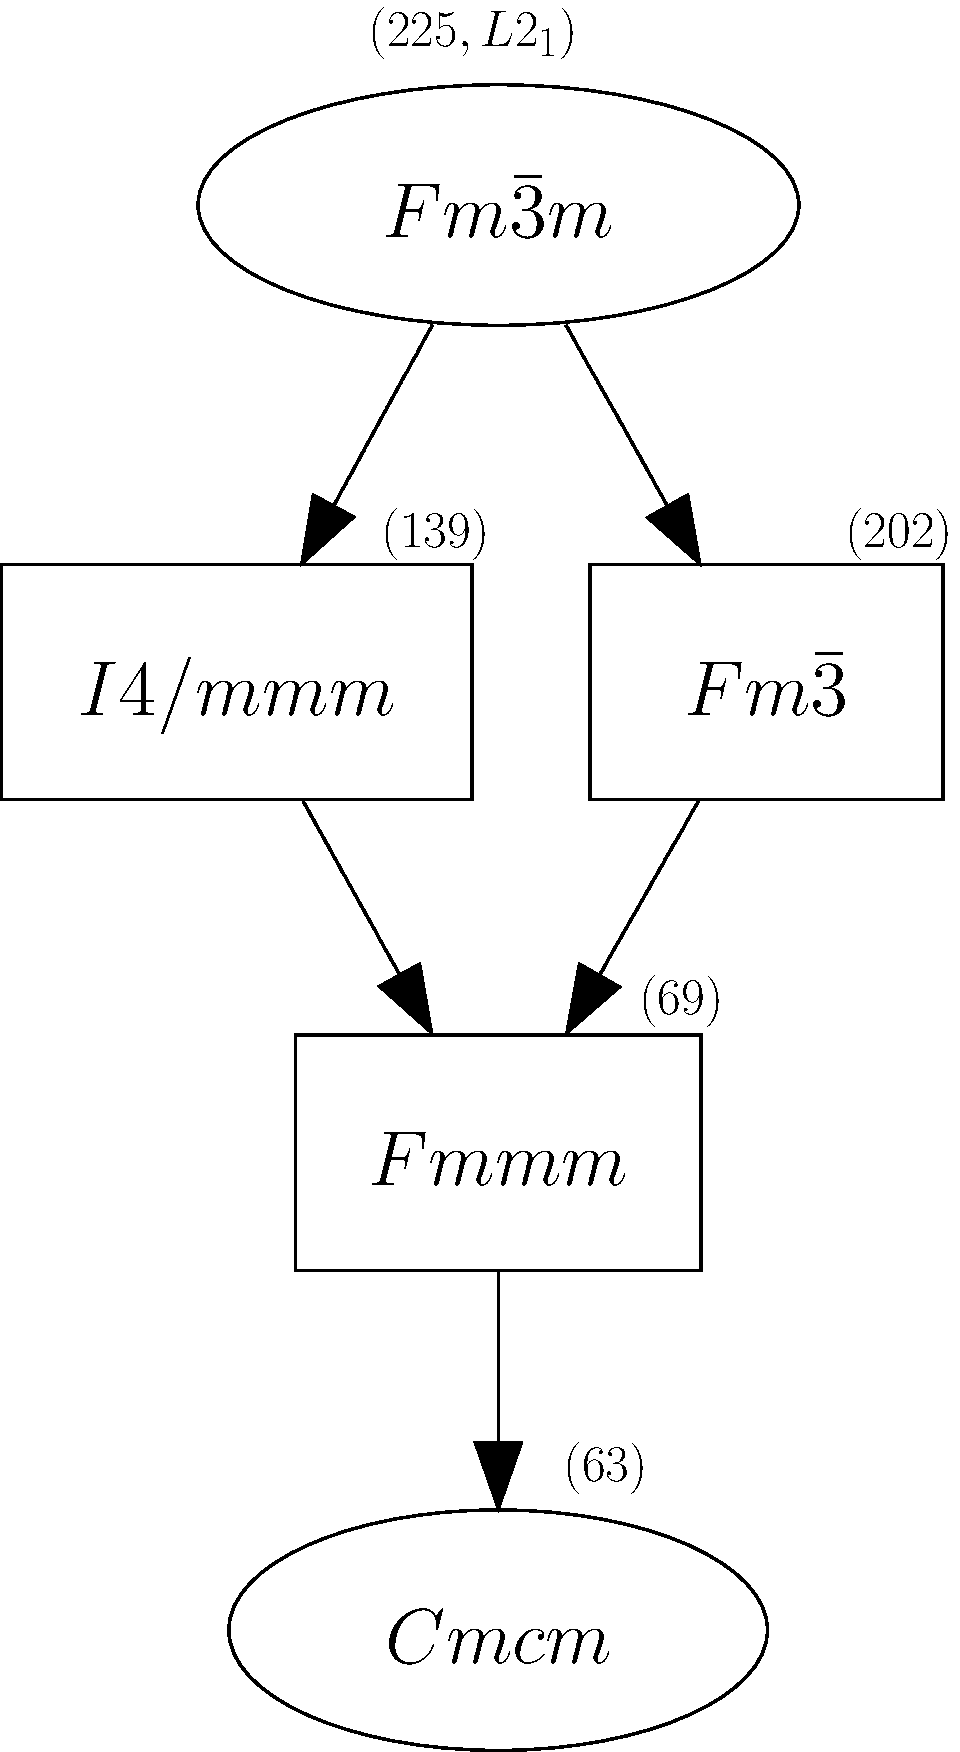
\includegraphics[scale=0.25]{figure_4c}}
  \hspace{1em}
\subfigure[ $ L2_1 $ - $ I\bar{4}m2 , 119 $ ]{
  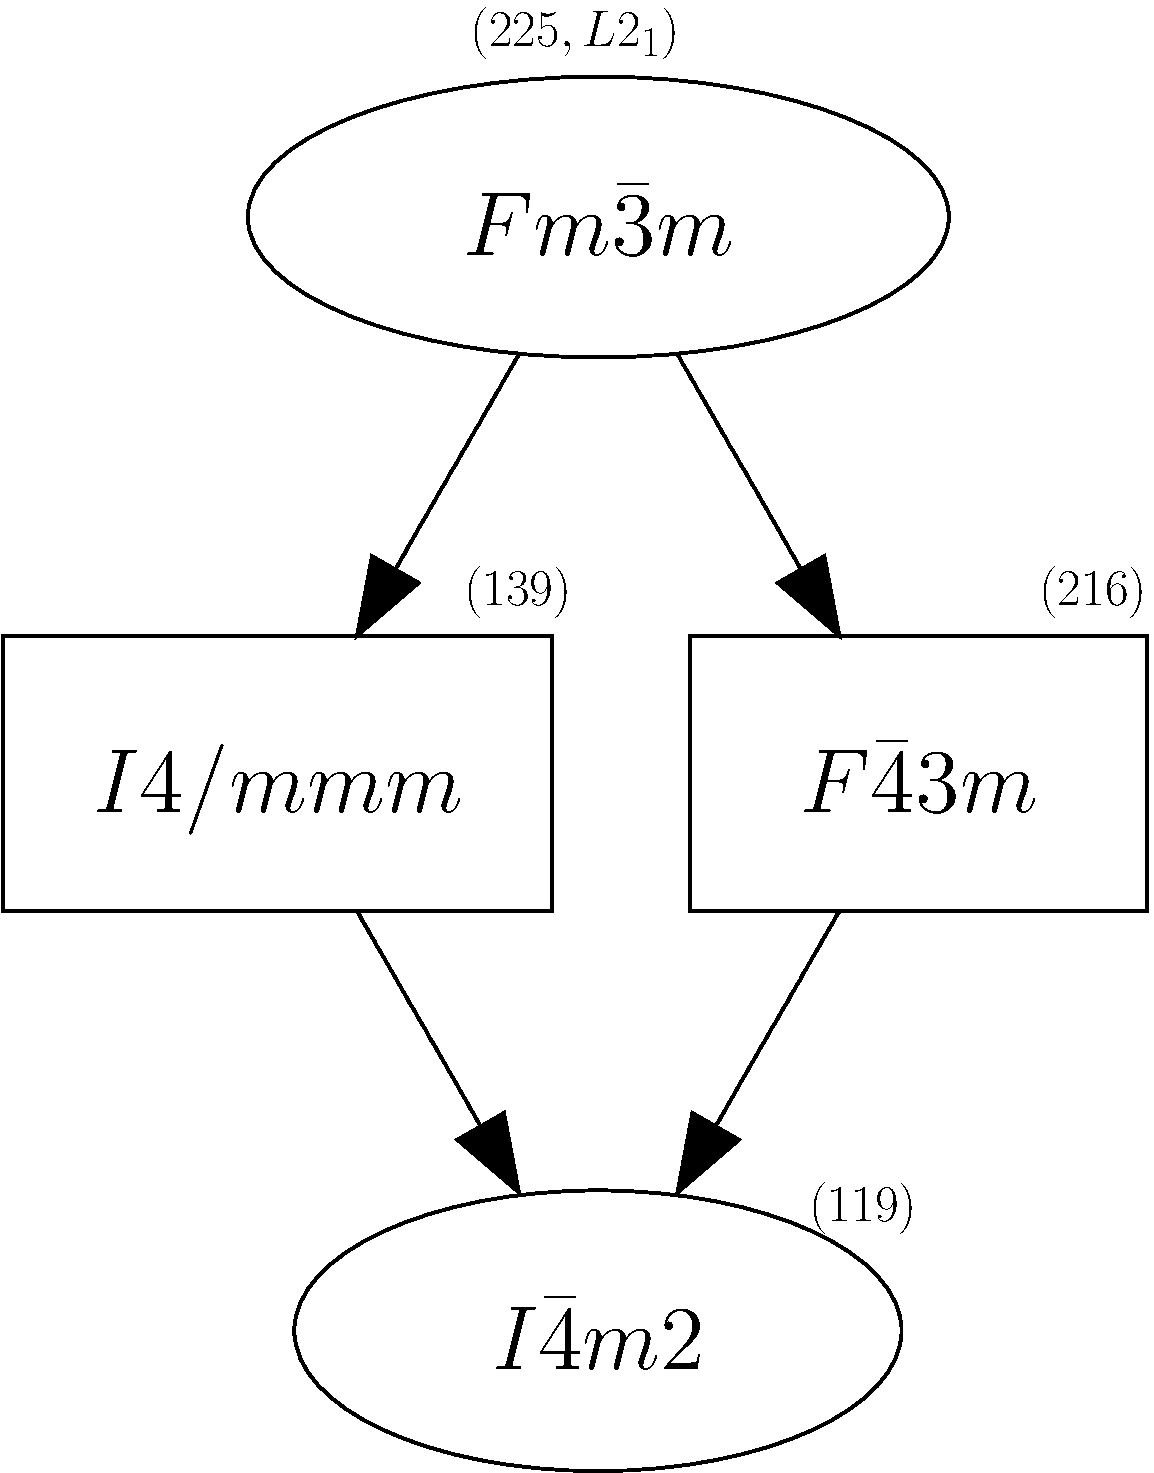
\includegraphics[scale=0.25]{figure_4d}}
\caption{Group-subgroup graphs for the transformations (a) $L2_1$-$O$ and (b)) $L2_1$-$L1_0$  and for space groups (c) 63 and (d) 119  as obtained in Table \ref{tab:minima_hopping} generated using the Bilbao crystallographic database. Space groups corresponding to the relevant point groups are indicated.}
\label{subgroups}
\end{figure}

As mentioned earlier, the austenitic phase in the Heusler system Co$_2$NiGa has a $L2_1$ structure. The martensitic transformation exhibited by this alloy is reversible, giving rise to the shape memory effect. This implies that the resultant martensite has a symmetry which is a sub-group of the austenitic cubic structure \cite{bhattacharya1998theory}.  The point group symmetries of the relevant structures are  $Fm\bar{3}m$.  for $L2_1$,  $P4/mmm$ for $L1_0$, and $Pmmn$ for the $O$ phase.  The point groups of both the $L1_0$ and the $O$  structures are sub-groups of the $L2_1$  point group. The group - subgroup relationship for the (a) $L2_1$-$O$ and  (b) $L2_1$-$L1_0$ are shown in Figs. \ref{subgroups}a and \ref{subgroups}b. Three possible paths  exist for the symmetry transformation from $L2_1$ to $O$ while two paths exist for the symmetry transformation from $L2_1$ to $L1_0$. Some examples of group-subgroup relations for additional structures isolated using the minima hopping method, which are close in energy to the $O$ structure, viz., structures corresponding 
to space groups $\#63$  and $\#119$, have been described in Figs. \ref{subgroups}c and \ref{subgroups}d. For both of these structures, we have two possible symmetry-reducing transformations. Of all the structures listed in Table \ref{tab:minima_hopping}, structures with space groups 12, 51, 59, 63, 119, 123 and 139 satisfy the symmetry relations with number of symmetry paths ranging between 1 and 5. For space groups 8 and 11, symmetry relations are satisfied, but the number of symmetry paths is 15 and 12, respectively. A larger number of possible symmetry paths amounts to a one to many correspondence, which makes it harder for a material to "remember" it's original crystal structure, thereby hindering the ideal shape memory effect. The remaining structures (space groups 3, 5, 31, 40, 44 ) do not satisfy the symmetry requirements. Thus, from a crystallographic point of view, it is seen that in addition to the $O$ phase,a number of other structures also satisfy requirements.

The ideal reversible martensitic transformation must also be a volume-preserving transition \cite{bhattacharya1998theory} since the higher the volume change, the greater is the hysteresis or irreversibility associated with the transformation. Having established the fact that there is a group-subgroup relation between $L2_1$  and the $O$ phase, we proceeded to investigate the existence of possible barriers to the transformation. Table  \ref{tab:volume} shows the volume change ($\delta V$) associated with the $L2_1$-$O$ and  $L2_1$-$L1_0$ transformations , the effective bulk modulus for the transformation ($B_e$) , the corresponding volumetric strain energy per unit volume ($E_v$), and the total energy for the transformation ($E_t$).  
The volumetric strain energy was calculated as
\begin{equation}
E_v = \frac{1}{2} \sigma_v \epsilon_v = \frac{1}{2} (B_e \epsilon_v ) \epsilon_v = \frac{1}{2} B_e {\epsilon_v}^2
\end{equation}
where $\sigma_v$ is the volumetric stress and $\epsilon_v$ is the volumetric strain. $\epsilon_v$ was calculated by taking the ratio of change in volume ($\delta V$) to original volume. $B_e$ was estimated by averaging the bulk moduli for the austenitic and martensitic phases. In Table  \ref{tab:volume}, it is apparent that the volumetric strain energy associated with the $L2_1$ - $O$ is about 5 times larger than that for the  $L2_1$ - $L1_0$ transformation; 
however when compared to the $E_t$, it it seen that its contribution is negligible. Also, one must keep in mind that bulk effects (such as those associated with elastic strain energy) only become important as the system volume becomes large enough. The possible nucleation of the $O$ phase from a parent $L2_1$ matrix is thus not ruled out.

\begin{table}
\begin{center}
\caption{Energy difference due to volume changes during transformation. Indicated are the volume change ($\delta V$) for the transformations , the effective bulk modulus for the transformation ($B_e$) , the corresponding volumetric strain energy per unit volume ($E_v$) and the total energy for the transformation ($E_t$).}
\setlength{\tabcolsep}{0.8cm}
\begin{tabular}{ccccc}
\hline
Transformation& $\delta V$ & $B_e$ &  $E_v$  & $E_t$ \\ 
 & ($\SI{}{\angstrom}^3$) &  (GPa)&   ($meV/ f.u$)& ($meV/ f.u$)  \\
\hline\hline
$L2_1$ - $O$ \ &  -0.28&   145&  -0.784  & -226.838 \\
\vspace{0.5em}
 $L2_1$ - $L1_0$ & -0.12 &   142.5 & -0.141 & -108.402  \\
\hline
\end{tabular}
\label{tab:volume}
\end{center}
\end{table}


\subsection{The phase selection problem}
 \begin{figure}[htp!]
  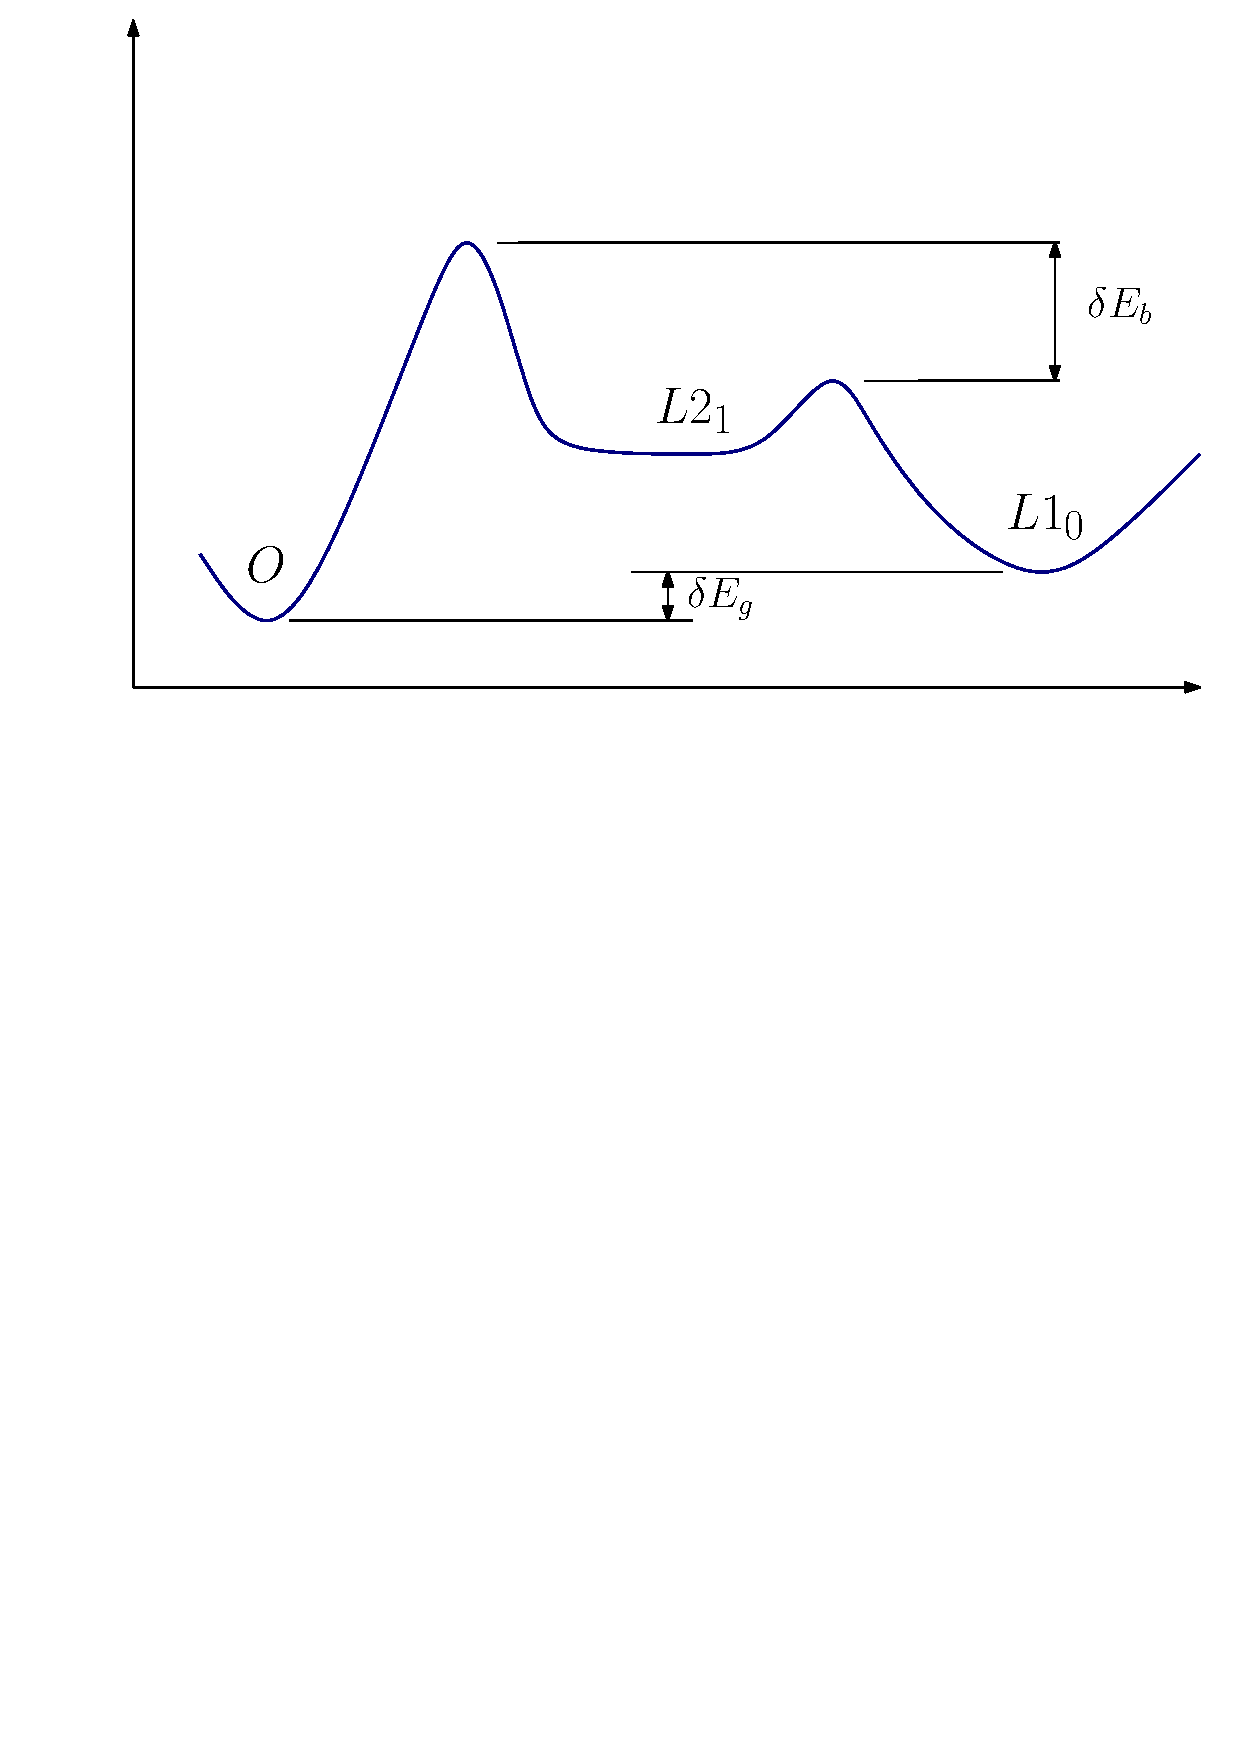
\includegraphics[scale=0.7]{figure_5}
  \caption{Schematic of relative stabilities of  the $L1_0$ and the $O$ structures in the Co-Ni-Ga heusler alloy. $\delta E_g$ is the energy difference between the conventional martensitic phase $L1_0$ and the $O$ phase. $\delta E_b$ is the proposed difference between the energy barriers for the $L2_1$- $ O$ transformation and the  $L2_1$ - $L1_0$ transformation.}
  \label{phase_selection}
\end{figure}
Recapitulating, the Co$_2$NiGa Heusler alloy shows a phase transformation from the austenitic, high-temperature $L2_1$ structure to the martensitic, low-temperature non-modulated $L1_0$ phase.  Minima hopping calculations predict a number of structures with monoclinic, tetragonal and orthorhombic symmetries with energies much lower than the $L1_0$ structure. Furthermore, Burgers path calculations  predict the existence of a martensitic phase with orthorhombic symmetry , the $ O $ phase. This phase is stable against perturbations along a Burgers transformation in a barrier-less fashion. While the examination of possible elastic energy barriers to the transformation suggested that there maybe some elastic constraints to the stabilization of the $O$ phase, the elastic energy may not be sufficient to completely rule it out.  

It is proposed that the absence of the $O$ phase may be attributed to the problem of phase selection. As seen in  Fig.\ref{phase_selection} ,  a possibility exists that while the $O$ phase is relatively more stable than the $L1_0$ phase , the energy barrier for the $L2_1$ -$O$ transformation may be higher than the barrier to the $L2_1$ -$L1_0$ transformation, i.e, $\delta E_b$ $>$  $\delta E_g$ at some temperature far away from the ground state conditions, when the system is cooled from the $L2_1$ structure. In this case, the high temperature austenitic phase  may not be able to sample a subset of low energy states since there may be no accessible paths. We proceeded to examine the stability of the $O$ phase in terms of its vibrational spectrum, its elastic constant tensor and we also examined the effect of configurational and magnetic disorder (brought about by high temperatures) on the competition between Bain and Burgers paths, taking the $L2_1$ structure into either the observed $L1_0$ or the missing $O$ 
phase.
.
\subsection{Phase stability analysis}

\subsubsection{Vibrational properties}
Phonon calculations were carried out to study the relative stability of the $L2_1$, $L1_0$, and $O$ structures. We used the FITFC module as implemented in the ATAT package to perform the vibrational calculations. This method consists of slightly perturbing the positions of the atoms away from their equilibrium position and calculating the reaction forces by fitting a spring model. Equating the calculated forces to the forces predicted from the harmonic model yields a set of linear constraints that allows the unknown force constants to be determined. The force constant matrix is then used to extract the projected vibrational density of states and the  phonon dispersion curves. The projected vibrational density of states is shown in Fig. \ref{CNG_pvdos} . 

\begin{figure}[htp!]
  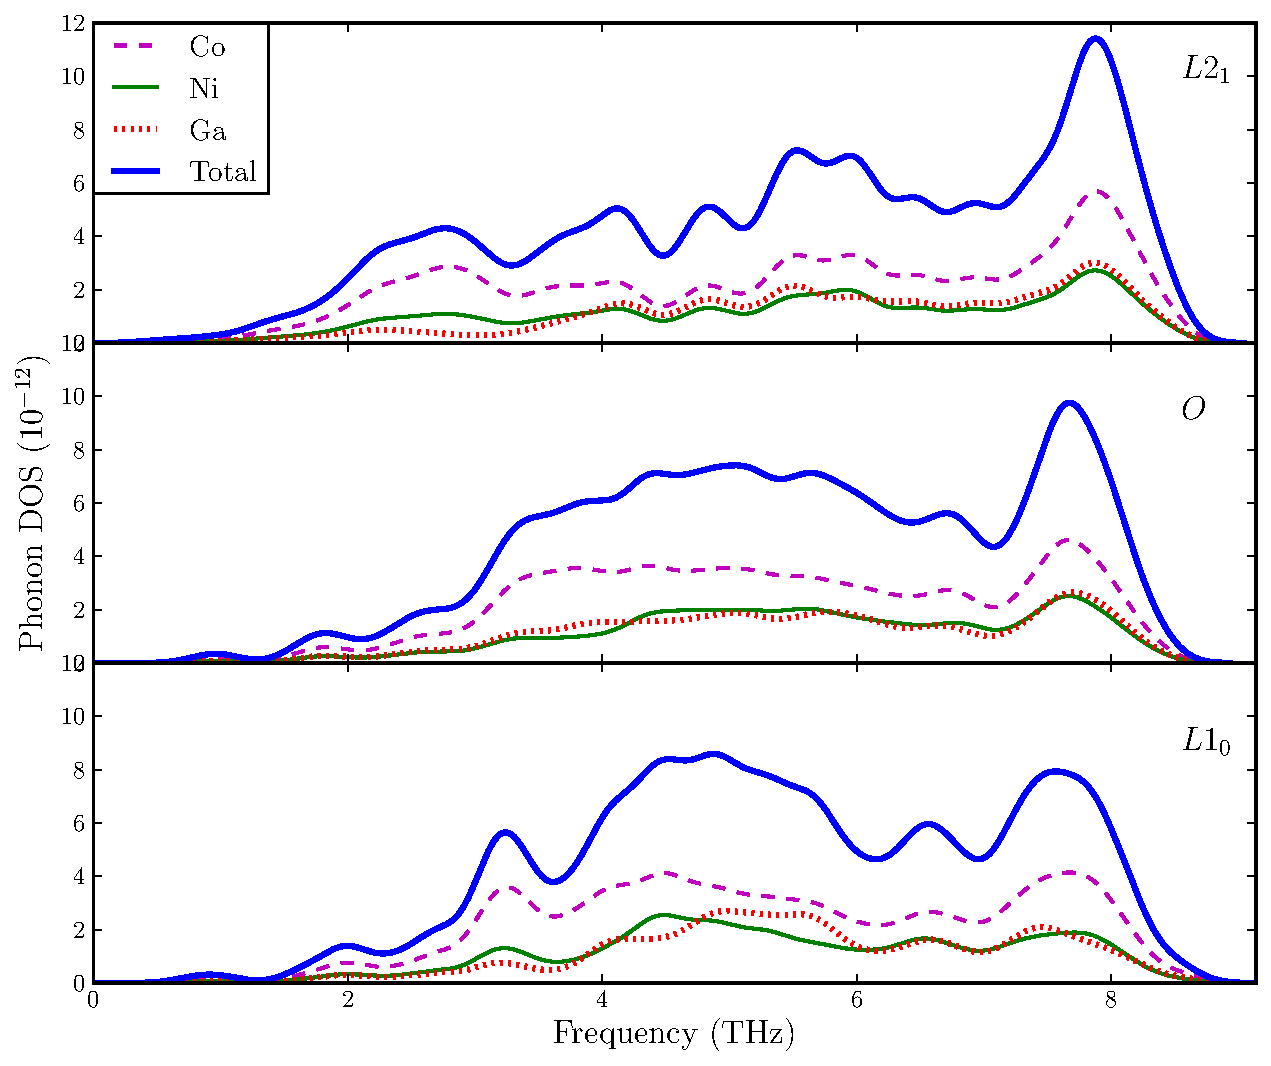
\includegraphics[scale=0.7]{figure_6}
  \caption{Projected vibrational density of states for the $Co_2NiGa$ system at $T=0$ K.}
  \label{CNG_pvdos}
\end{figure}

\begin{figure}
  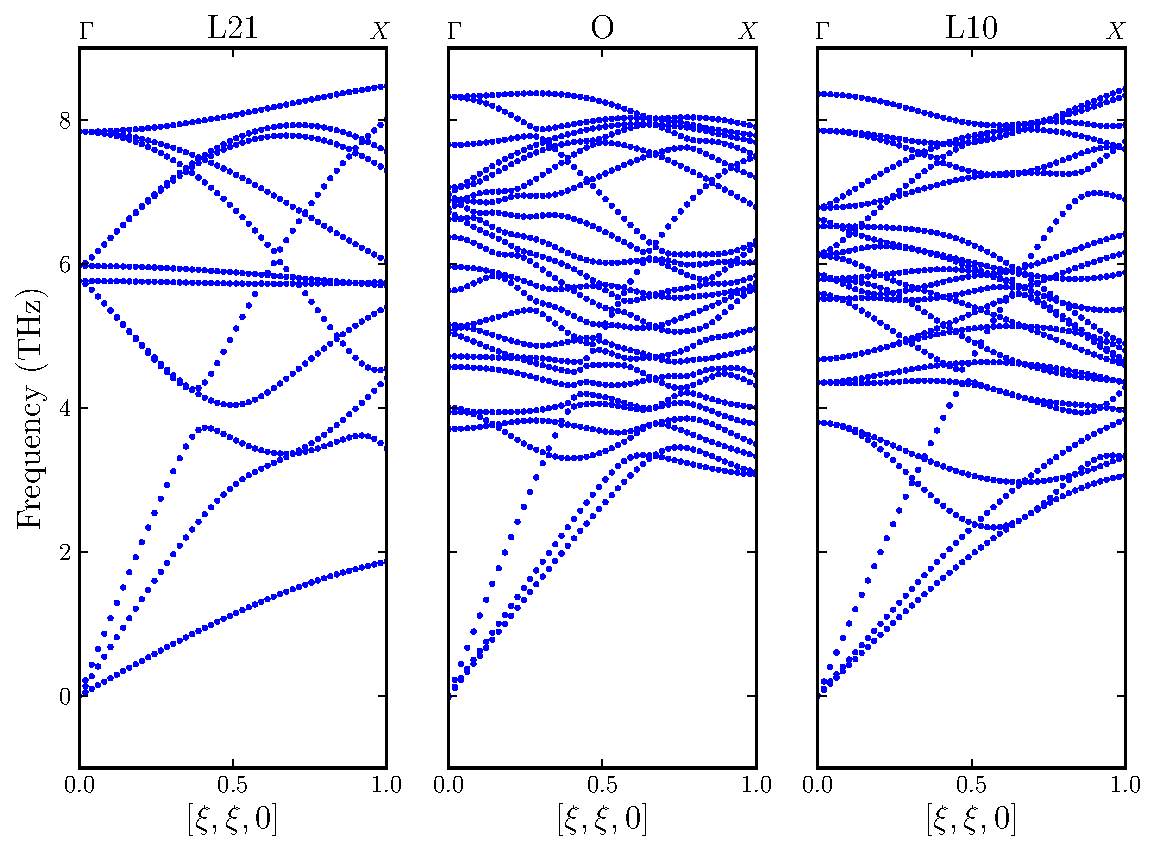
\includegraphics[scale=0.7]{figure_7}
  \caption{Phonon dispersion curves  along the $[\xi,\xi,0] $ direction for the $Co_2NiGa$ system at $T=0$ K. }
  \label{CNG_dispersion}
\end{figure}

The mode of interest in these alloys is along the $[110]$ direction. The calculated phonon dispersion curves of the three structures were compared. Fig. \ref{CNG_dispersion}  shows the projected vibrational density of states for these structures along the $[\xi,\xi,0] $ directions in the Co$_2$NiGa  systems. No unstable modes are observed. Softening of the optical modes is observed in the $L1_0$ as well as the $O$ structures. No conclusions can be drawn about the relative stability of the structures. The vibrational contribution to the total energy was estimated for the three structures by integrating over the vibrational density of states. However, the contributions were negligible ( $< 5 $meV); hence we do not include them in this work.

\subsubsection{Elastic properties}
\label{subsec:elastic}
\begin{table}
\begin{center}
\caption{Calculated elastic properties of $CoNiGa$  in GPa : significant components of the stiffness tensor ($C_{ij}$), bulk modulus (B), shear modulus (G), elastic modulus (E) and Poisson's ratio ($\nu$). Calculations were performed using the GGA \cite{Perdew1992} approximation. }
\begin{tabular}{clccccccccc}
\hline
Alloy& Structure& \ $c_{11}$ \ & \ $c_{12}$ \ & \ $c_{13}$ \ & \ $c_{33}$ \ & \ $c_{44}$ \ & \ $B$ \ & \ $G$ \ & \ $E$ \ & \ $\nu$ \ \\
\hline\hline
$CoNiGa$ \ &$L2_1$ & 181  & 186 & 186 & 181 & 141 &136  &52 &139  &0.33 \\
\vspace{0.5em}
 \ & $L1_0$ & 252 & 153 & 163 & 204 & 114 &149  &71  & 184 &0.29 \\
 \vspace{0.5em}
 \ & O & 265 & 154 &108 & 328 & 55  &154  &66  &173  &0.31 \\
\hline
\end{tabular}
\label{tab:elastic}
\end{center}
\end{table}

Elastic constants for the structures considered in this work were calculated  as explained in Sec. \ref{Sec:computational_details} and are listed in Table \ref{tab:elastic} in GPa. Included are the significant components of the stiffness tensor ( $c_{11}$ , $c_{12}$ , $c_{13}$ , $c_{33}$  and  $c_{44}$) , bulk modulus ($B$), shear modulus ($G$), elastic modulus ($E$), and Poisson's ratio ($\nu$). From the table we see that the elastic moduli of $L1_0$ and $O$ structures are close in magnitude. There is no suggestion of instability. $C_{11}-C_{12}$  lends an insight into the stability of the structure with respect to shear and other martensitic transformation inducing deformations. For the $L2_1$ structure,  $C_{11}-C_{12}$  $<$ $0$, which is expected since the $L2_1$ structure is  unstable with respect to temperature and undergoes a martensitic transformation. However $C_{11}-C_{12}$  values for both $L1_0$ and $O$ structures are positive,  with the value for the $O$ phase being higher indicating increased stability with respect to the $L1_0$ structure.


\subsection{Effect of disorder on the competition between Bain and Burgers paths} 

While arguments using rough estimates for the elastic strain energy associated with the $L2_1-L1_0$ and $L2_1-O$ transformations suggest a higher elastic barrier for the latter, these arguments cannot be used when looking at the incipient process of the formation of a new phase out of the $L2_1$ matrix since at early stages of the phase transformation bulk energy contributions may not be significant enough. On the other hand, the phonon and elastic calculations suggest that the $O$ phase is mechanically stable. This leads us to believe that there exist mechanisms arising from hitherto unaccounted for contributions within the material which make these low energy states inaccessible when coming from high-temperature experiments. We thus proceed to examine three such contributions: (i) the effect of configurational disorder, (ii) magnetic disorder, and (iii) atomic disorder.

\subsubsection{Effect of configurational disorder}

\begin{figure}[htp!]
  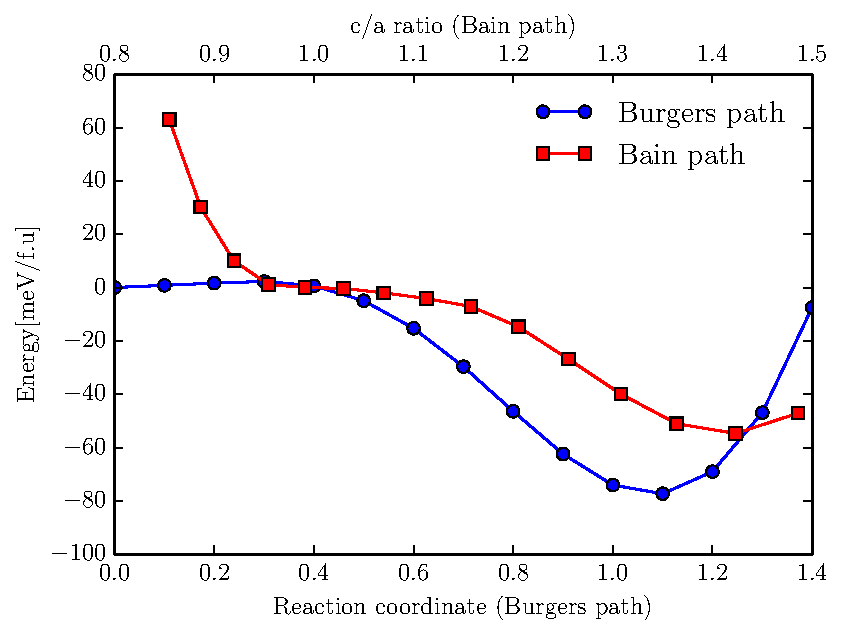
\includegraphics[scale=1.0]{figure_8}
  \caption{Energy profile comparison for Bain and single parameter Burger  paths in  disordered (SQS) $Co_2NiGa$}
  \label{SQS}
\end{figure}

It is well known that atomic ordering may influence the transformation behavior of SMAs. Substantial experimental and numerical work has been carried out in investigating the order-disorder transition, long-range ordering, and effect of ordering on the phase transformation characteristics in various shape memory alloys \cite{singh2011effect,Obradobccstability1997,recarte2012dependence}. Recarte \textit{et al.} show that in Ni-Mn-In SMA, the thermodynamics of the martensitic transformation depends on the atomic ordering \cite{recarte2012dependence}.
The effect of configurational disorder was simulated by using special quasirandom structures (SQS)  \cite{zunger1990special}, implemented using the ATAT toolkit. A 32-atom supercell was used and the Bain and Burgers paths were recalculated for this structure and are shown in Fig. \ref{SQS}. We see that the energy at the minimum along the Bain path is still higher than that along the Burgers path, although the energy difference is substantially lowered ($\approx 25 meV $). 

\subsubsection{Effect of magnetic disorder}
\label{mag_disorder}
 In this sub-section, we present  Bain path and Burgers path calculations for varying degrees of magnetization ($100 \% - 0 \%)$.  This may be viewed as a crude method to simulate the effect of high temperatures  by lowering the magnetization. This is achieved by using the fixed spin moments method within VASP. Specifically, we assign a value to the parameter ‘NUPDOWN’ in the INCAR file. Fixing the value of this parameter ensures that the difference of the number of electrons in the up and down spin component will be kept fixed to the specified value. We calculate the Bain and Burgers paths for the different values of NUPDOWN. For these calculations, VASP automatically sets MAGMOM = NUPDOWN/number of ions; hence we use the term ‘MAGMOM’ to denote the different cases. Results are presented for 100 $\%$,  90 $\%$, 70 $\%$, 50 $\%$, 30 $\%$  magnetic moment values and the non-magnetic case. 

    \begin{figure}[htp!]
\subfigure[MAGMOM = $100 \%$]{
  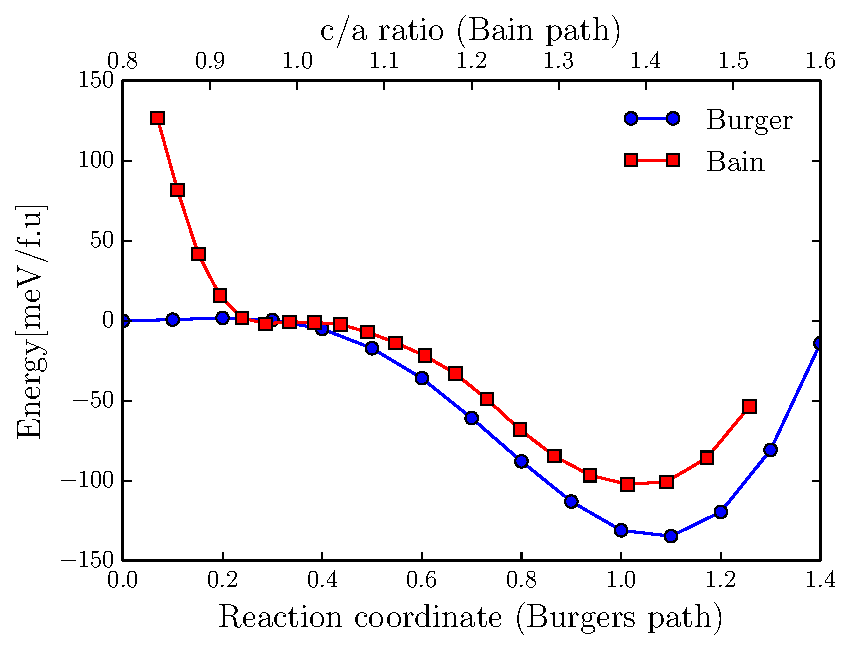
\includegraphics[scale=0.5]{figure_9a}}
\subfigure[MAGMOM = $90 \%$]{
  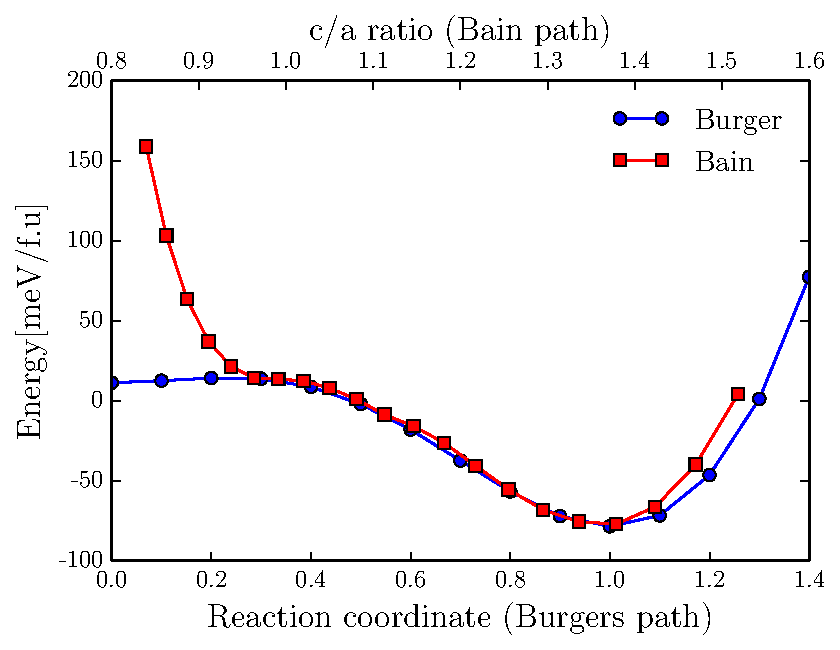
\includegraphics[scale=0.5]{figure_9b}}
\subfigure[MAGMOM = $70 \%$]{  
  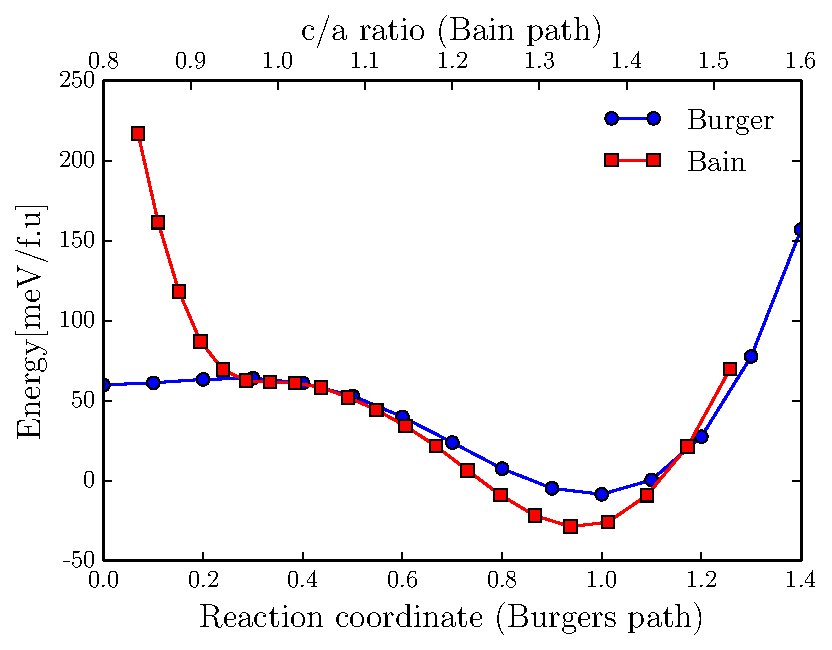
\includegraphics[scale=0.5]{figure_9c}}
  \subfigure[MAGMOM = $50 \%$]{
  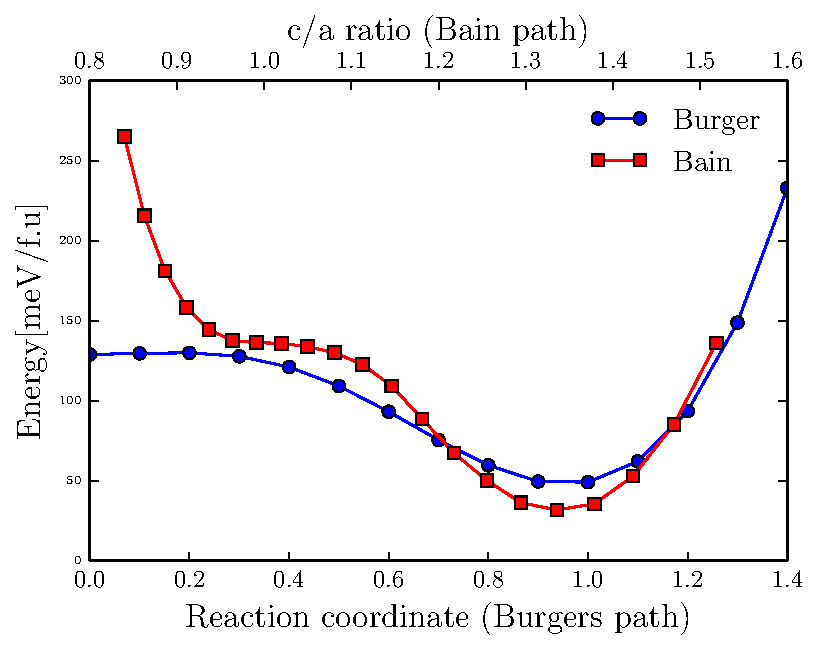
\includegraphics[scale=0.5]{figure_9d}}
\subfigure[MAGMOM = $30 \%$]{  
  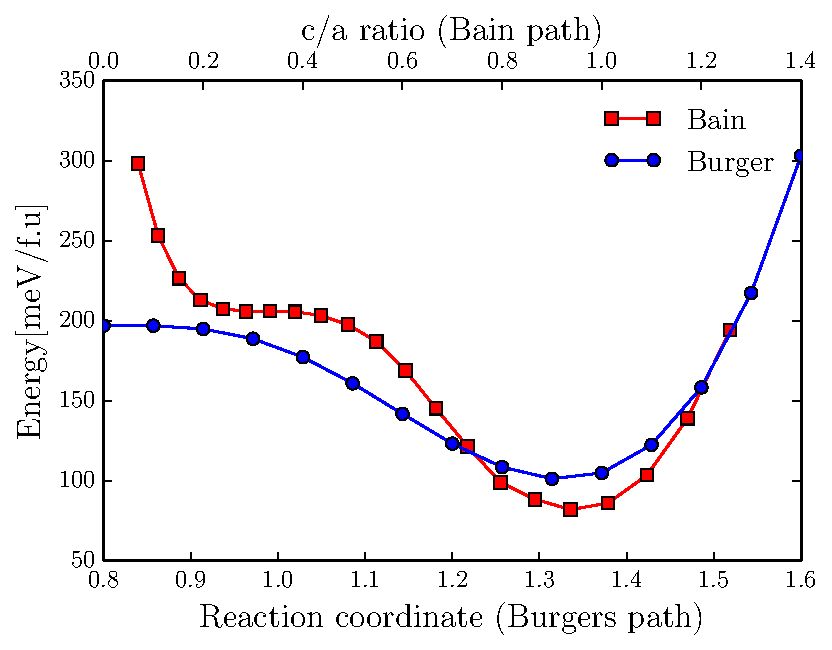
\includegraphics[scale=0.5]{figure_9e}}
\subfigure[non-magnetic]{  
  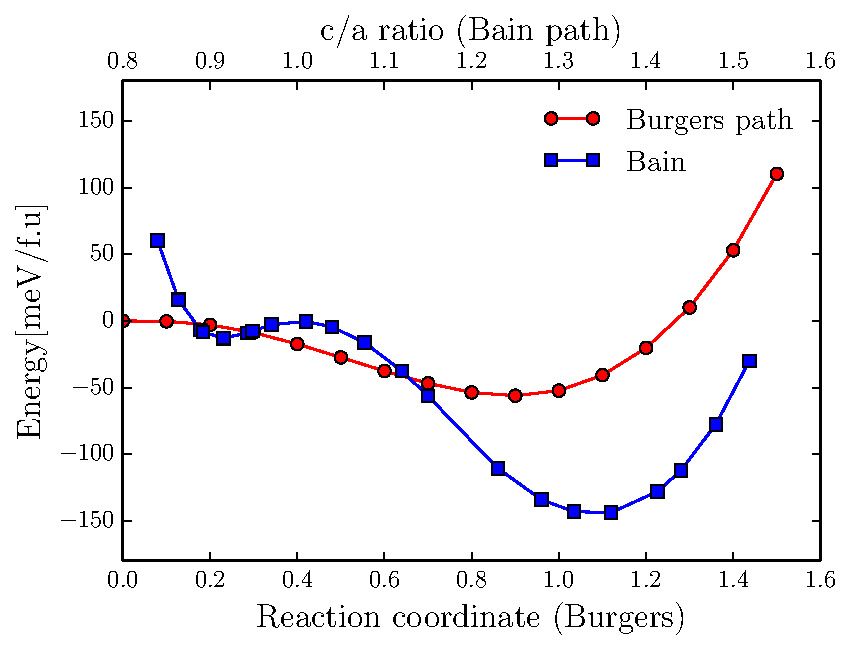
\includegraphics[scale=0.5]{figure_9f}}

\caption{Energy profile comparison for Bain and single-parameter Burgers paths in  $Co_2NiGa$  for varying values of magnetization (fixed spin moment calculations). }
\label{magnetic_disorder}
\end{figure}

In Fig. \ref{magnetic_disorder}, it is seen that for the 100 $\%$ MAGMOM case,  as seen before, the Burgers path has a lower minima than the Bain path; i.e., the $O$ phase is more stable than the $L1_0$ phase. However, on lowering the magnetic moment,  as in Fig. \ref{magnetic_disorder} (b), the Burgers and Bain paths have almost coinciding minima. On further lowering the magnetic moment  as in Fig. \ref{magnetic_disorder}(c) - \ref{magnetic_disorder}(f), the trend is reversed and the Bain path is seen to have an increasingly lower minima than the Burgers path.  Thus reducing the magnetization of the system, i.e., introducing magnetic disorder and simulating the effect of higher temperatures, stabilizes the $L1_0$ phase with respect to the $O$ phase. 
%%----------------------------------------------------------------------------------------------------------------------------------------------------------------------------------------------------------%%
\subsubsection{Effect of non-stoichiometric composition}

\begin{figure}[htp!]
  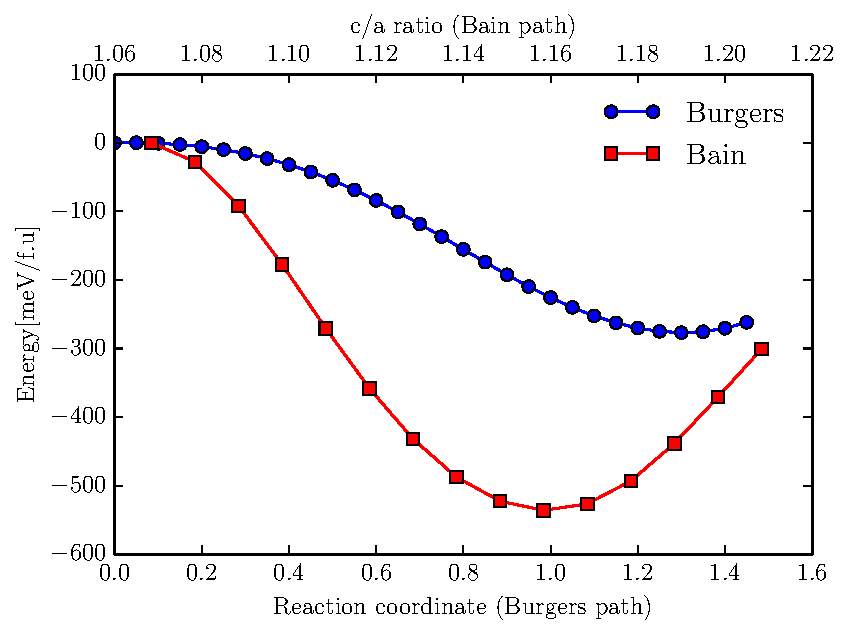
\includegraphics[scale=1.0]{figure_10}
  \caption{Energy profile comparison for Bain and single-parameter Burgers paths in   $Co_7Ni_4Ga_5$.}
  \label{fig:non_stoic}
\end{figure}
In this section we account for the effect of atomic disorder, viz, the modeling of the transformation in  a non-stoichiometric composition. As observed in \cite{siewert2010electronic}, it is not 
simple to  achieve the perfect Heusler composition $Co_2NiGa$  because one is very near the two-phase ($\gamma+\beta)$ region or at the border  of the $B2$ 
phase. Simulating a non - stoichiometric composition also weakens the magnetic ordering naturally ( as opposed to fixed-spin calculations in Sec. 
\ref{mag_disorder}). We use a 16-atom SQS supercell to model the the $Co_{43.75}Ni_{25}Ga_{31.25}$  composition and calculate the Bain path. Since the symmetry of the structure is lowered due to the off - stoichiometric composition, the Bain path (varying of c/a) was calculated for 2 cases: (i) $c || z$ and (ii) $c || y$.  We then selected the Bain path with the lower energy profile. For the Burgers path, we used a simple 16-atom supercell to simulate the structure. Since Ga replaces Co, we considered all possible configurations of Ga replacing Co and then selected the lowest energy configuration. The Burgers path was carried out on the lowest energy configuration.
Thus it was ensured that the lowest possible Bain path and Burgers paths were used, which encapsulate all possible energy ranges which may be observed and enable us to make a qualitative, if not quantitative observation.
The results are indicated in Fig. \ref{fig:non_stoic}. It is seen that the $L1_0$  structure as achieved through the Bain path is more stable than the corresponding $O$ phase for this composition. This may be attributed to the weakening of the magnetic ordering due to substitution of one $Co$ atom by a  $Ga$ atom, as mentioned earlier .
%%----------------------------------------------------------------------------------------------------------------------------------------------------------------------------------------------------------%%
\section{Summary and Conclusion}
\label{Sec:summary}
 The Burgers path was investigated in the Co-Ni-Ga ferromagnetic shape memory alloy system. Calculations were carried out using two models: a single-parameter characterization of the Burgers path and a two-parameter Burgers model which generates a transformation energy surface. In both models, a low-energy structure with an orthorhombic symmetry ($O$) is observed whose parameters are shifted from the expected co-ordinates for the transformation. This low energy structure ($O$) has been unobserved experimentally. Complete relaxation of the $O$ structure shows further reduction in energy. The Bain path for the alloys is also determined and compared to the Burgers path. Minima hopping calculations were carried out to investigate the energy landscapes surrounding the $L1_0$ martensitic phase in $Co -  Ni - Ga$. Results showed the existence of a number of structures similar in energy to  as well as much lower than the predicted $O$ phase in the vicinity of the $L1_0$ structure. It was postulated the the Co$_2$NiGa  Heusler 
system exhibits a classic case of the phase selection problem. Although the  unexpected $O$phase may be relatively more stable than the $L1_0$ phase,  the energy barrier for the $L2_1$ -$O$ transformation may be much higher than the barrier to the $L2_1$ -$L1_0$ transformation.  This high barrier 
may be due to vibrational effects, elastic effects, configurational disorder, magnetic disorder, or due to micro-structural effects.  

In an effort to validate this hypothesis, the stability of this structure was investigated via elastic and lattice dynamics calculations  and the contributions of configurational and magnetic disorder on the transformations were studied.  No instabilities due to vibrational effects were detected. Elastic calculations showed comparable values of elastic properties for the $L1_0$ and $O$ phases.  $C_{11}-C_{12}$ values showed that the $O$ phase is relatively more stable than the $L1_0$ phase. Calculations incorporating configurational disorder showed a lowering in the energy difference between the $L1_0$ and the $O$ structures, but the $O$ structure was still more stable. The calculations simulating the effect of magnetic disorder/ high temperature showed that the $L1_0$ structure may be stabilized with respect to the $O$ phase by lowering the magnetic moment. Thus,  it is proposed that magnetic disorder plays an important role in the phase selection energetics of the $CoNiGa$ system and is a principal contributor in the determination of the transformation path followed in this system. Further calculations were carried out on an off-stoichiometric composition $Co_{43.75}Ni_{25}Ga_{31.25}$ , where the weakening of the magnetic ordering manifests naturally. As expected, the $L1_0$ phase was seen to be more stable than the $O$ phase.

Reverting to the question raised in Sec. \ref{Sec:intro},  we conclude that  it is  unrealistic to use standard DFT prototypes to investigate ground states of relatively  less known systems. By performing a detailed analysis of the transformation paths (Burgers and Bain) by taking into account perturbations on the ground state, it is seen that what is manifested is in principle a phase selection problem: the ultimate crystal structure that the system transforms into, depends on the path that the system prefers. When coming from high temperature, the accessible path is that corresponding to  the Bain transformation. To conclude, discrepancies between DFT and experiments may be reconciled if we consider the  "history" of the alloy.
%%----------------------------------------------------------------------------------------------------------------------------------------------------------------------------------------------------------%%
\section*{Acknowledgments}
R. A. and A.T. acknowledge support from NSF through Grants No. CMMI-0953984, No. DMR-0805293, and No. DMR-DMR-0844082 [International Institute for Multifunctional Materials for Energy Conversion-(IIMEC)]. First-principles calculations by R.A. and A.T. were carried out in the Chemical Engineering Cluster and the Texas A\& M Supercomputing Facility at Texas A\&M University as well as the Texas Advanced Computing Center (TACC) at the University of Texas at Austin. Preparation of the input files and analysis of the data have been performed within the framework  of AFLOW/ACONVASP developed by Stefano Curtarolo as well as with the ATAT package developed by Axel van de Walle. A. T. would like to acknowledge the contribution of  Mario Siewart towards preliminary calculations.
We also acknowledge the support from the Extreme Science and Engineering Discovery Environment (XSEDE), which is supported by National Science Foundation Grant No. ACI-1053575. P.E. acknowledges support by Deutsche Forschungsgemeinschaft (Priority Programme SPP 1599). A.H.R. and I.V-J. acknowledge support from CONACYT under Project No. 152153. AHR also acknowledges the support of NSF through DMREF-NSF 1434897 and the donors of the American Chemical Society Petroleum Research Fund for partial support of this research under contract No. 54075-ND10. We are thankful to M. Amsler and S. Goedecker for useful discussions and the use of  their minima hopping implementation.	
%%----------------------------------------------------------------------------------------------------------------------------------------------------------------------------------------------------------%%
\bibliography{CoNiGa_stability}
%%----------------------------------------------------------------------------------------------------------------------------------------------------------------------------------------------------------%%
\end{document}
